\documentclass[a4paper, 11pt]{article}
\usepackage[utf8]{inputenc}
\usepackage[english,russian]{babel}
\usepackage[T1, T2A]{fontenc}
\usepackage{graphicx}
\usepackage{multirow}
\usepackage{pgfplots}
\pgfplotsset{compat=1.9}
\usepackage[left = 2cm, right = 2cm, bottom = 2cm, top = 2cm]{geometry}
\usepackage{listings}
\usepackage{threeparttable}
\usepackage[tableposition=top]{caption}
\usepackage{subcaption}
\DeclareCaptionLabelFormat{gostfigure}{Рисунок #2}
\DeclareCaptionLabelFormat{gosttable}{Таблица #2}
\DeclareCaptionLabelSeparator{gost}{~---~}
\captionsetup{labelsep=gost}
\captionsetup[figure]{labelformat=gostfigure}
\captionsetup[table]{labelformat=gosttable}
\renewcommand{\thesubfigure}{\asbuk{subfigure}}
\captionsetup[table]{labelformat=simple, labelsep = endash, justification = raggedright, singlelinecheck = off}
\usepackage{indentfirst}

\graphicspath{{image/}}

\usepackage[top=2cm, left=2cm, right=2cm, left=2cm]{geometry}
\usepackage{amsmath}

\graphicspath{{image/}}

\newcommand\tline[2]{$\underset{\text{#1}}{\text{\underline{\hspace{#2}}}}$}

\begin{document}
	\begin{titlepage}
		\centering
		{\fontsize{12pt}{5cm}\selectfont \bfseries Министерство образования и науки Российской Федерации} \\ \vspace{0.5cm}
		{\fontsize{7pt}{5cm}\selectfont ФЕДЕРАЛЬНОЕ ГОСУДАРСТВЕННОЕ АВТОНОМНОЕ ОБРАЗОВАТЕЛЬНОЕ УЧРЕЖДЕНИЕ ВЫСШЕГО ПРОФЕССИОНАЛЬНОГО ОБРАЗОВАНИЯ} \\ 
		\vspace{1cm}
		{\fontsize{12pt}{5cm}\selectfont \bfseries САНКТ-ПЕТЕРБУРГСКИЙ УНИВЕРСИТЕТ ИНФОРМАЦИОННЫХ ТЕХНОЛОГИЙ, МЕХАНИКИ И ОПТИКИ} \\ \vspace{1.5cm}

		{\fontsize{14pt}{5cm}\selectfont Кафедра \hspace{1cm} \underline{Систем Управления и Информатики}  \hspace{1cm} Группа \underline{Р3340}} \\ 
		\vspace{2cm}

		{\fontsize{20pt}{5cm}\selectfont \bfseries Лабораторная работа №7} \\
		{\fontsize{20pt}{5cm}\selectfont \bfseries “Анализ точности систем управления”} \\
		{\fontsize{14pt}{5cm}\selectfont Вариант - 7} \\
		\vspace{1.5cm}

		\flushleft

		{Выполнил \hspace{2cm} \tline{(фамилия, и.о.)}{9cm} (подпись)} \\
		\vspace{2cm}

		{Проверил \hspace{2cm} \tline{(фамилия, и.о.)}{9cm} (подпись)} \\
		\vspace{5cm}

		"\underline{\hspace{0.7cm}}"\hspace{0.2cm}\underline{\hspace{2cm}}\hspace{0.2cm}20\underline{\hspace{0.7cm}}г. \hspace{2cm} Санкт-Петербург, \hspace{2cm} 20\underline{\hspace{0.7cm}}г. \\ \vspace{1cm}

		Работа выполнена с оценкой \hspace{1cm} \underline{\hspace{8cm}} \\ 
		\vspace{1cm}
		Дата защиты "\underline{\hspace{0.7cm}}"\hspace{0.2cm}\underline{\hspace{2cm}}\hspace{0.2cm}20\underline{\hspace{0.7cm}}г.

\end{titlepage}

\begin{center}
\section*{Задание}
\end{center}
\subsection*{Цель работы}
Исследование точностных свойств систем управления путём воздействия на систему различных типовых воздействий, а также внешних возмущений. Для характеристики точностных свойств системы надо определить предельное значение установившейся ошибки.


\subsection*{Исходные данные}
\begin{table}[h!]
\centering
\begin{threeparttable}
\caption{Исходные данные}\label{tab:perflogcross}
\begin{tabular}{|c|c|c|c|c|c|c|c|}
\hline
$W(s)(0)$ & $W(s)(1)$ & $A$ & $V$ & $a$ & $f_1$ & $f_2$ & $g(t)$\\
\cline{1-8}
\rule{0cm}{0.75cm}
\(\displaystyle \frac{1}{2s^2+3s+1}\) & \(\displaystyle \frac{s+1}{2s^2+3s+1}\) & 1 & 1.5 & 0.25 & -0.25 & 1 & $3+0.6sin(0.4t)$\\[0.4cm]
\hline

\end{tabular}
\end{threeparttable}
\end{table}

\newpage
\begin{center}
\section{Исследование системы с астатизмом нулевого порядка}
\end{center}

\begin{figure}[h]
\center{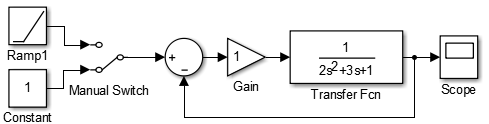
\includegraphics[width=0.75\linewidth]{1.png}}
\caption{Структурная схема моделируемой системы}
\label{ris:image}
\end{figure}

\subsection{Исследование стационарного режима работы}

\pgfplotsset{
every axis plot post/.append style={
	mark= ,
	every mark/.append style={solid},
	every axis title/.style={at={(0.5,0)},anchor=north,yshift=-0.1}
	}}
\par
На рисунке 2 представлены графики $y(t)$ при различных значениях $k$ в стационарном режиме $g(t)=1$.
\begin{figure}[h!]
\centering
\begin{tikzpicture}
\begin{axis}[
	xmin = 0,
	ymin = 0,
	xmax = 30,
	xlabel = {\Large{$t,c$}},
	ylabel = {\Large{$y$}},
	width = 300,
	height = 250,
	grid = both,
	extra y ticks = { 0.5, 0.91, 0.83},
	extra y tick style={grid style={black, line width = 1}},
	ytick = {0, 0.2, 0.4, 0.6, 1, 1.2}
]

\addplot[line width = 2] table [x=t, y=y] 
              {data/1_1_k_1.txt};
\addplot[line width = 2, loosely dashed,draw = red] table [x=t, y=y]
			{data/1_1_k_5.txt};
\addplot[line width = 2, dotted, draw = blue] table [x=t, y=y]
			{data/1_1_k_10.txt};

\legend{
	$k=1$,
	$k=5$,
	$k=10$	
	}
\end{axis}
\end{tikzpicture}
\caption{Результаты моделирования при $g(t)=1$}
\end{figure}

Для стационарной системы при постоянном входном воздействии $g(t)=A$ предельное значение установившейся ошибки можно найти:
\begin{equation}
\varepsilon=\frac{A}{1+k}
\end{equation}
\par
Таким образом, найдём ошибки при разных значениях $k$:
\par
$\varepsilon=0.5(k=1)$, $\varepsilon\approx0.17(k=5)$, $\varepsilon=0.09(k=10)$
\par
Графики ошибок приведены на рисунке 3.
\begin{figure}[h!]
\centering
\begin{tikzpicture}
\begin{axis}[
	legend pos = north east, 
	xmin = 0,
	xmax = 30,
	xlabel = {\Large{$t,c$}},
	ylabel = {\Large{$e(t)$}},
	width = 300,
	height = 250,
	grid = both,	
	extra y ticks = { 0.5, 0.17, 0.09},
	extra y tick style={grid style={black, line width = 1}},
	ytick = {-0.2, 0.4, 0.6, 0.8, 1}
]

\addplot[line width = 2] table [x=t, y=e_1] 
              {data/1_1_e.txt};
\addplot[line width = 2, loosely dashed, draw = red] table [x=t, y=e_5]
			{data/1_1_e.txt};
\addplot[line width = 2, dotted, draw = blue] table [x=t, y=e_10]
			{data/1_1_e.txt};

\legend{
	$k=1$,
	$k=5$,
	$k=10$	
	}
\end{axis}
\end{tikzpicture}
\caption{Графики ошибок}
\end{figure}

\newpage
\subsection{Исследование режима движения с постоянной скоростью}

\par
На рисунке 4 представлены графики $y(t)$ при различных значениях $k$ в режиме движения с постоянной скоростью $g(t)=1.5t$.
\begin{figure}[h!]
\centering
\begin{tikzpicture}
\begin{axis}[
	legend pos = north west, 
	xmin = 0,
	ymin = 0,
	xmax = 30,
	xlabel = {\Large{$t,c$}},
	ylabel = {\Large{$y$}},
	width = 300,
	height = 250,
	grid = both,
]

\addplot[line width = 2] table [x=t, y=y] 
              {data/1_2_k_1.txt};
\addplot[line width = 2, loosely dashed, draw = red] table [x=t, y=y]
			{data/1_2_k_5.txt};
\addplot[line width = 2, dotted, draw = blue] table [x=t, y=y]
			{data/1_2_k_10.txt};

\legend{
	$k=1$,
	$k=5$,
	$k=10$	
	}
\end{axis}
\end{tikzpicture}
\caption{Результаты моделирования при $g(t)=1.5t$}
\end{figure}

Как видно из полученных графиков, ошибка постоянно растёт, не имея какого-то установившегося значения.
\par
Графики ошибок представлены на рисунке 5.
\newpage

\begin{figure}[h!]
\centering
\begin{tikzpicture}
\begin{axis}[
	legend pos = north east, 
	xmin = 0,
	xmax = 30,
	xlabel = {\Large{$t,c$}},
	ylabel = {\Large{$e(t)$}},
	width = 300,
	height = 250,
	grid = both,	
	%extra y ticks = { 0.5, 0.17, 0.09},
	%extra y tick style={grid style={black, line width = 1}},
	%ytick = {-0.2, 0.4, 0.6, 0.8, 1}
]

\addplot[line width = 2] table [x=t, y=e_1] 
              {data/1_2_e.txt};
\addplot[line width = 2, loosely dashed, draw = red] table [x=t, y=e_5]
			{data/1_2_e.txt};
\addplot[line width = 2, dotted, draw = blue] table [x=t, y=e_10]
			{data/1_2_e.txt};

\legend{
	$k=1$,
	$k=5$,
	$k=10$	
	}
\end{axis}
\end{tikzpicture}
\caption{Графики ошибок}
\end{figure}

\newpage
\begin{center}
\section{Исследование системы с астатизмом первого порядка}
\end{center}

\begin{figure}[h]
\center{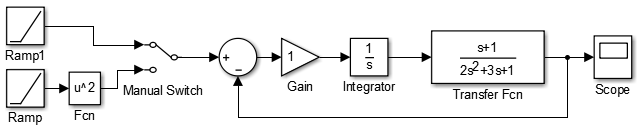
\includegraphics[width=0.75\linewidth]{2.png}}
\caption{Структурная схема моделируемой системы}
\label{ris:image}
\end{figure}

\subsection{Исследование стационарного режима работы}

\par
На рисунке 7 представлены графики $y(t)$ при различных значениях $k$ в стационарном режиме $g(t)=1$.
\begin{figure}[h!]
\centering
\begin{tikzpicture}
\begin{axis}[
	xmin = 0,
	ymin = 0,
	xmax = 30,
	xlabel = {\Large{$t,c$}},
	ylabel = {\Large{$y$}},
	width = 300,
	height = 250,
	grid = both,
]

\addplot[line width = 2] table [x=t, y=y] 
              {data/2_1_k_1.txt};
\addplot[line width = 2, loosely dashed, draw = red] table [x=t, y=y]
			{data/2_1_k_5.txt};
\addplot[line width = 2, dotted, draw = blue] table [x=t, y=y]
			{data/2_1_k_10.txt};

\legend{
	$k=1$,
	$k=5$,
	$k=10$	
	}
\end{axis}
\end{tikzpicture}
\caption{Результаты моделирования при $g(t)=1$}
\end{figure}

\par
В стационарном режиме система с астатизмом первого порядка имеет нулевую ошибку. Графики ошибок представлены на рисунке 8.

\begin{figure}[h!]
\centering
\begin{tikzpicture}
\begin{axis}[
	legend pos = north east, 
	xmin = 0,
	xmax = 30,
	xlabel = {\Large{$t,c$}},
	ylabel = {\Large{$e(t)$}},
	width = 300,
	height = 250,
	grid = both,	
	%extra y ticks = { 0.5, 0.17, 0.09},
	%extra y tick style={grid style={black, line width = 1}},
	%ytick = {-0.2, 0.4, 0.6, 0.8, 1}
]

\addplot[line width = 2] table [x=t, y=e_1] 
              {data/2_1_e.txt};
\addplot[line width = 2, loosely dashed, draw = red] table [x=t, y=e_5]
			{data/2_1_e.txt};
\addplot[line width = 2, dotted, draw = blue] table [x=t, y=e_10]
			{data/2_1_e.txt};

\legend{
	$k=1$,
	$k=5$,
	$k=10$	
	}
\end{axis}
\end{tikzpicture}
\caption{Графики ошибок}
\end{figure}

\newpage
\subsection{Исследование режима движения с постоянной скоростью}

\par
На рисунке 9 представлены графики $y(t)$ при различных значениях $k$ в режиме движения с постоянной скоростью $g(t)=1.5t$.
\begin{figure}[h!]
\centering
\begin{tikzpicture}
\begin{axis}[
	xmin = 0,
	ymin = 0,
	legend pos = north west,
	xmax = 30,
	xlabel = {\Large{$t,c$}},
	ylabel = {\Large{$y$}},
	width = 300,
	height = 250,
	grid = both,
]

\addplot[line width = 2] table [x=t, y=y] 
              {data/2_2_k_1.txt};
\addplot[line width = 2, loosely dashed, draw = red] table [x=t, y=y]
			{data/2_2_k_5.txt};
\addplot[line width = 2, dotted, draw = blue] table [x=t, y=y]
			{data/2_2_k_10.txt};
\addplot[line width = 2, draw = orange]{1.5*x};

\legend{
	$k=1$,
	$k=5$,
	$k=10$,
	$g(t)$
	}
\end{axis}
\end{tikzpicture}
\caption{Результаты моделирования при $g(t)=1.5t$}
\end{figure}

Предельное значение установившейся ошибки для системы с астатизмом первого порядка при $g(t)=Vt$:
\begin{equation}
\varepsilon=\frac{V}{k}
\end{equation}
\par
Таким образом, найдём ошибки для различных значений $k$:
\par
$\varepsilon=1.5(k=1)$, $\varepsilon=0.3(k=5)$, $\varepsilon=0.15(k=10)$
\par
Графики ошибок представлены на рисунке 10.

\begin{figure}[h!]
\centering
\begin{tikzpicture}
\begin{axis}[
	legend pos = north east, 
	xmin = 0,
	xmax = 30,
	xlabel = {\Large{$t,c$}},
	ylabel = {\Large{$e(t)$}},
	width = 300,
	height = 250,
	grid = both,	
	extra y ticks = {0.3, 0.15},
	extra y tick style={grid style={black, line width = 1}},
	ytick = {-0.5, 0.5, 1, 1.5, 2, 2.5}
]

\addplot[line width = 2] table [x=t, y=e_1] 
              {data/2_2_e.txt};
\addplot[line width = 2, loosely dashed, draw = red] table [x=t, y=e_5]
			{data/2_2_e.txt};
\addplot[line width = 2, dotted, draw = blue] table [x=t, y=e_10]
			{data/2_2_e.txt};

\legend{
	$k=1$,
	$k=5$,
	$k=10$	
	}
\end{axis}
\end{tikzpicture}
\caption{Графики ошибок}
\end{figure}

\newpage
\subsection{Исследование режима движения с постоянным ускорением}

\par
На рисунке 11 представлены графики $y(t)$ при различных значениях $k$ в режиме движения с постоянным ускорением $g(t)=0.25t^2$.
\begin{figure}[h!]
\centering
\begin{tikzpicture}
\begin{axis}[
	xmin = 0,
	ymin = 0,
	legend pos = north west,
	xmax = 30,
	xlabel = {\Large{$t,c$}},
	ylabel = {\Large{$y$}},
	width = 300,
	height = 250,
	grid = both,
]

\addplot[line width = 2] table [x=t, y=y] 
              {data/2_3_k_1.txt};
\addplot[line width = 2, loosely dashed, draw = red] table [x=t, y=y]
			{data/2_3_k_5.txt};
\addplot[line width = 2, dotted, draw = blue] table [x=t, y=y]
			{data/2_3_k_10.txt};

\legend{
	$k=1$,
	$k=5$,
	$k=10$	
	}
\end{axis}
\end{tikzpicture}
\caption{Результаты моделирования при $g(t)=0.25t^2$}
\end{figure}

Ошибка при \(\displaystyle g(t)=\frac{at^2}{2}\) стремится к бесконечности.
\par
Графики ошибок представлены на рисунке 12.

\newpage

\begin{figure}[h!]
\centering
\begin{tikzpicture}
\begin{axis}[
	legend pos = north west, 
	xmin = 0,
	xmax = 30,
	xlabel = {\Large{$t,c$}},
	ylabel = {\Large{$e(t)$}},
	width = 300,
	height = 250,
	grid = both,	
	%extra y ticks = {0.3, 0.15},
	%%extra y tick style={grid style={black, line width = 1}},
	%ytick = {-0.5, 0.5, 1, 1.5, 2, 2.5}
]

\addplot[line width = 2] table [x=t, y=e_1] 
              {data/2_3_e.txt};
\addplot[line width = 2, loosely dashed, draw = red] table [x=t, y=e_5]
			{data/2_3_e.txt};
\addplot[line width = 2, dotted, draw = blue] table [x=t, y=e_10]
			{data/2_3_e.txt};

\legend{
	$k=1$,
	$k=5$,
	$k=10$	
	}
\end{axis}
\end{tikzpicture}
\caption{Графики ошибок}
\end{figure}

\newpage
\begin{center}
\section{Исследование влияния внешних возмущений}
\end{center}

\par
На рисунке 13 представлены графики $y(t)$ при различных значениях возмущающих воздействий $f_1$ и $f_2$.
\begin{figure}[h]
\center{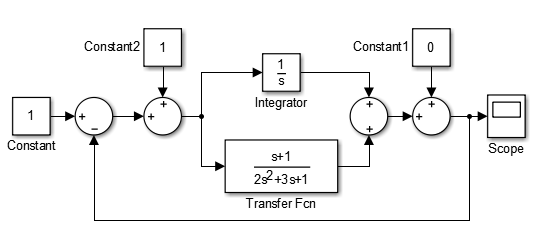
\includegraphics[width=0.75\linewidth]{3.png}}
\caption{Структурная схема моделируемой системы}
\label{ris:image}
\end{figure}

\begin{figure}[h!]
\centering
\begin{tikzpicture}
\begin{axis}[
	legend pos = south east,
	xmin = 0,
	ymin = 0,
	xmax = 30,
	xlabel = {\Large{$t,c$}},
	ylabel = {\Large{$y$}},
	width = 300,
	height = 250,
	grid = both,
]

\addplot[line width = 2] table [x=t, y=y] 
              {data/3_2.txt};
\addplot[line width = 2, loosely dashed, draw = red] table [x=t, y=y]
			{data/3_3.txt};

\legend{
	$f_1=-0.25$,
	$f_2=1$	
	}
\end{axis}
\end{tikzpicture}
\caption{Результаты моделирования при $g(t)=1$}
\end{figure}

Ошибка для данной системы будет иметь следующий вид:
\begin{equation}
e(s)=-\left(\frac{3s^2+4s+1}{2s^3+6s^2+5s+1}f_2-\frac{2s^3+3s^2+s}{2s^3+6s^2+5s+1}f_1\right)
\end{equation}
\par
При стремлении s к нулю получаем следующее значение искомой ошибки:\\
$\varepsilon=-f_2$\\
$\varepsilon=0(f_1=-0.25, f_2=0)$\\
$\varepsilon=-1(f_1=0, f_2=1)$
\par
Графики ошибок представлены на рисунке 14.

\newpage
\begin{figure}[h!]
\centering
\begin{tikzpicture}
\begin{axis}[
	legend pos = north east, 
	xmin = 0,
	xmax = 30,
	xlabel = {\Large{$t,c$}},
	ylabel = {\Large{$e(t)$}},
	width = 300,
	height = 250,
	grid = both,	
	%extra y ticks = {0.3, 0.15},
	%%extra y tick style={grid style={black, line width = 1}},
	%ytick = {-0.5, 0.5, 1, 1.5, 2, 2.5}
]

\addplot[line width = 2] table [x=t, y=e_1] 
              {data/3_2_e.txt};
\addplot[line width = 2, loosely dashed, draw = red] table [x=t, y=e_2]
			{data/3_2_e.txt};

\legend{
	$f_1=0 | f_2=1$,
	$f_1=-0.25 | f_2=0$	
	}
\end{axis}
\end{tikzpicture}
\caption{Графики ошибок}
\end{figure}

\newpage
\begin{center}
\section{Исследование установившейся ошибки при произвольном входном воздействии}
\end{center}

\begin{figure}[h]
\center{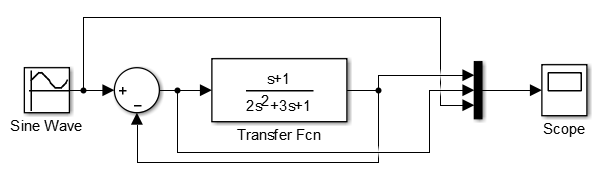
\includegraphics[width=0.75\linewidth]{4.png}}
\caption{Структурная схема моделируемой системы}
\label{ris:image}
\end{figure}
\par
На рисунке 17 представлены графики $y(t)$, $g(t)=3+0.6sin(0.4t)$ и $e(t)$.
\begin{figure}[h!]
\centering
\begin{tikzpicture}
\begin{axis}[
	legend pos = south east,
	xmin = 0,
	ymin = 0,
	xmax = 30,
	xlabel = {\Large{$t,c$}},
	ylabel = {\Large{$y$}},
	width = 300,
	height = 250,
	grid = both,
]

\addplot[line width = 2] table [x=t, y=y] 
              {data/4_1_y.txt};
\addplot[line width = 2, loosely dashed, draw = red] table [x=t, y=y]
			{data/4_1_g.txt};
\addplot[line width = 2, dotted, draw = blue] table [x=t, y=y]
			{data/4_1_e.txt};

\legend{
	$y(t)$,
	$g(t)$,
	$e(t)$	
	}
\end{axis}
\end{tikzpicture}
\caption{Результаты моделирования при $g(t)=3+0.6sin(0.4t)$}
\end{figure}

Найдём приближённое аналитическое выражение для $e(t)$:
\begin{equation}
e(t)=c_0g(t)+c_1\frac{d}{dt}g(t)+\frac{c_2}{2!}\frac{d^2}{dt^2}g(t)
\end{equation}
, где \(\displaystyle c_i=\frac{d^i}{dt^i}F_e(s)\)\\
\\
\(\displaystyle F_e(s)=\frac{1}{1+W(s)}=\frac{2s^2+3s+1}{2s^2+4s+2}\)
\\
\\
\\
$g'(t)=0.24cos(0.4t)$\\
$g''(t)=-0.096sin(0.4t)$\\
\\
$c_0=0.5$\\
$c_1=0.5$\\
$c_2=-1$\\
\begin{equation}
e(t)=1.5+0.12cos(0.4t)+0.348sin(0.4t)
\end{equation}
\par
На рисунке 18 представлены графики ошибок $e_{exp}(t)$ и $e_{anal}(t)$
\begin{figure}[h!]
\centering
\begin{tikzpicture}
\begin{axis}[
	legend pos = south east,
	xmin = 0,
	ymin = 0,
	xmax = 30,
	xlabel = {\Large{$t,c$}},
	ylabel = {\Large{$e(t)$}},
	width = 300,
	height = 250,
	grid = major,
]

\addplot[line width = 2] table [x=t, y=y] 
              {data/4_1_e.txt};
\addplot[line width = 2, loosely dashed, draw = red] table [x=t, y=y]
			{data/4_2_e_anal.txt};

\legend{
	$e_{exp}(t)$,
	$e_{anal}(t)$	
	}
\end{axis}
\end{tikzpicture}
\caption{Результаты моделирования экспериментальной и аналитически вычисленной ошибок}
\end{figure}

\par
Как видно из полученных графиков, расхождение экспериментальной и теоретической ошибок минимально, что позволяет использовать полученное выражение для исследования системы.
\newpage
\begin{center} 	
\section*{Выводы}
\end{center}
\par
В ходе лабораторной работы были исследованы системы с разными порядками астатизма и различными входными и возмущающими воздействиями. 
\par
Система с астатизмом нулевого порядка в стационарном режиме имеет тем меньшую ошибку, чем больше коэффициент пропорциональности $k$. В режиме движения с постоянной скоростью ошибка стремится к бесконечности.
\par
Для системы с астатизмом первого порядка в стационарном режиме ошибка равна нулю, а в режиме движения с постоянной скоростью ошибка равна константе, определяемой выражением $\frac{V}{k}$. В режиме движения с постоянным ускорением ошибка стремится к бесконечности.
\par
Для данной системы возмущение измерительного устройства не имеет значения, а возмущение по управлению равно ошибке.
\par
Для исследования ошибки системы при произвольном входном воздействии искомая ошибка была аналитически разложена на основе данных о системе и входном воздействии в ряд Тейлора. При сравнении теоретической и экспериментальной ошибок наблюдается достаточно точное совпадение графиков, поэтому аналитическое выражение для ошибки вполне можно использовать для исследования точностных характеристик системы с произвольным входным воздействием.
\end{document}
